\begin{titlepage}
   \begin{center}
       \vspace*{9cm}
       \LARGE
       \textbf{Unidad 2: Técnicas de Vacío}

      
   
            
       \vspace{0.8cm}
     
      
   \end{center}
\end{titlepage}
\section{Teoría Cinética de los gases}

\subsection{Propiedades de equilibrio}
 \begin{figure}
        \centering
        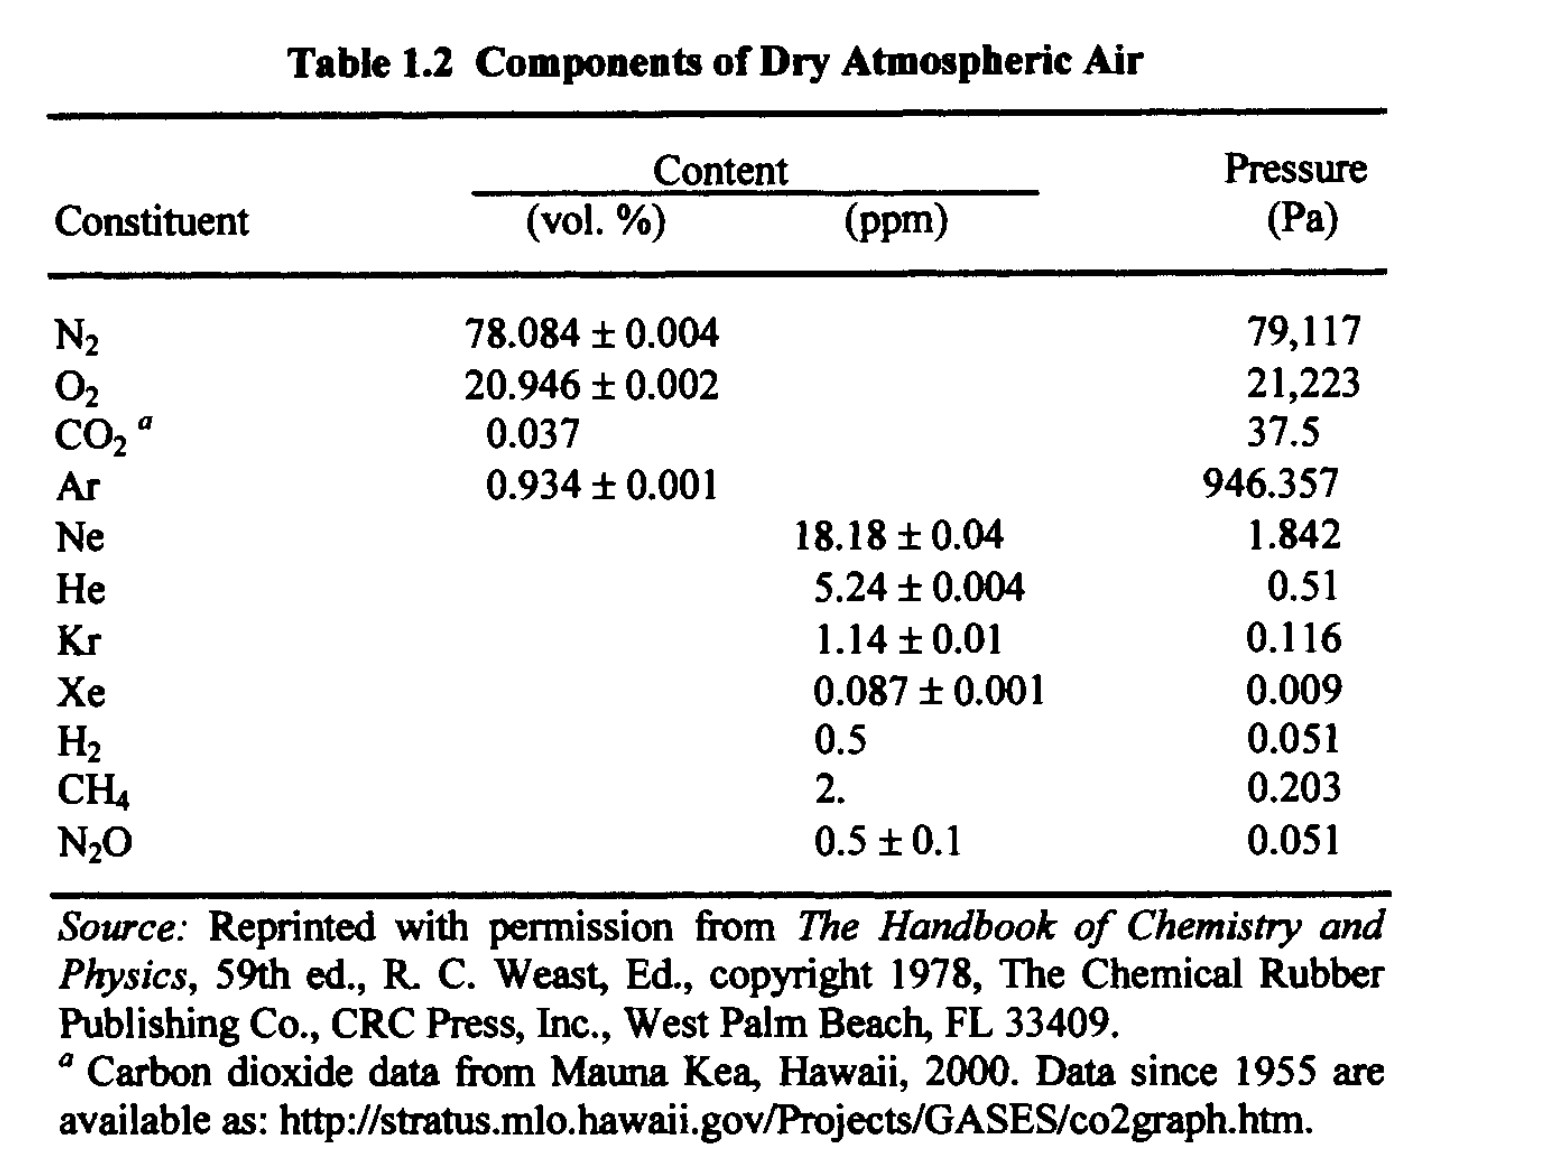
\includegraphics[width=0.75\textwidth]{Imagenes/Unidad/U2/Tabla composición del aire atmosférico.jpg}
        \caption{Tabla composición del aire atmosférico. Pregunta 1}
        \label{fig:my_label}
    \end{figure}

    \begin{figure}
        \centering
        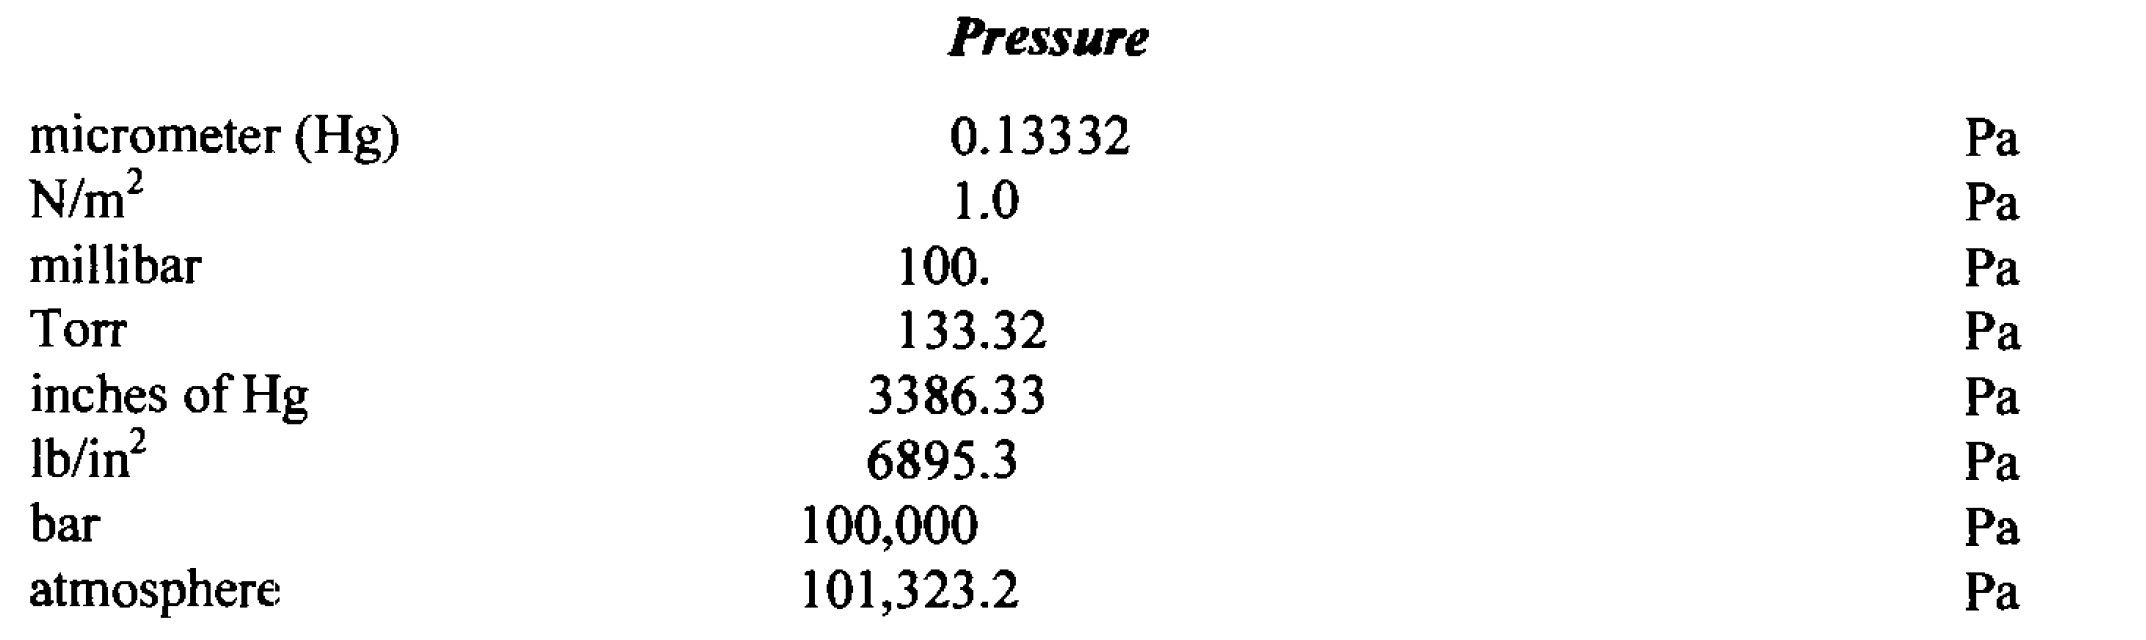
\includegraphics[width=0.75\textwidth]{Imagenes/Unidad/U2/Unidades de presion del libro.jpg}
        \caption{Unidades de presión. Pregunta 2}
        \label{fig:my_label}
    \end{figure}
\begin{enumerate}
    
    \setcounter{enumi}{2}
    \item %Pregunta 3 
    Velocidad promedio de las moléculas de un gas ideal en términos de la temperatura:
    \begin{equation}
        < v > = \sqrt{\frac{8k_B T}{m \pi}}
    \end{equation}
    donde $k_B$ es la constante de Boltzmann en Joules/Kelvin, $m$ es la masa de la partícula en kg, y $T$ la temperatura en Kelvin.
    \item %Pregunta 4
     La masa del nitrógeno molecular es  $ m = 2\cdot 2.3258671 \cdot 10^{-26}$  kg y la temperatura ambiente $T = 25$°C$= 298.15$ K. La constante de Boltzmann es $k_B = 1.38064910 \cdot 10^{-23}$ J/K. Así , la velocidad promedio es $v = 475 \pm 0.1$ m/s. Esta velocidad se relaciona con la velocidad del sonido ya que este último utiliza al aire como un medio de propagación.
     
\end{enumerate}
\subsection{Propiedades de transporte}
\begin{enumerate}[resume]
\item %Pregunta 5
% medida de la interacción entre proyectiles o partículas lanzadas contra un centro dispersor
El concepto de sección eficaz, como su nombre indica, se refiere al área efectiva para la colisión. La sección eficaz de un objetivo esférico es
\begin{equation}
    \sigma = 4 \pi r^2
\end{equation}
Sabiendo que el radio del nitrógeno es $r=1.55\cdot 10^{-10}$m. Su sección eficaz es $\sigma =7.5\cdot10^{-20} m^2$

\item % Pregunta 6
Debido que las moléculas están distribuidas de forma aleatoria y se mueven a distintas velocidades implica que recorren distintos “caminos libres”.  Así, el camino libre medio  $\lambda$ corresponde a la distancia promedio que recorre una partícula entre dos colisiones sucesivas. 


\item % Pregunta 7
El camino libre medio se expresa como
\begin{equation}
    \lambda =\frac{1}{ \sigma n_v} 
\end{equation}
donde $n_v$ es el número de moléculas por volumen. Por ley de los gases ideales $n_v = \frac{P}{K_BT}$. De esta forma, 

\begin{equation}
    \lambda = \frac{K_BT}{\sigma P }
\end{equation}
donde $K_B$ es la constante de Boltzmann, $T$ la temperatura, $P$ la presión y $\sigma$ la sección eficaz. 



\begin{figure}
    \centering
    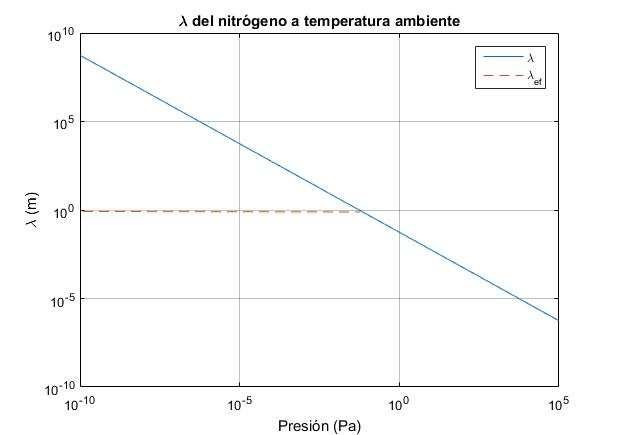
\includegraphics[width=0.55\textwidth]{Imagenes/Unidad/U2/grafp8.jpg}
    \caption{Camino libre medio para el nitrógeno. Preguntas 8 y 9}
    \label{fig:my_label}
\end{figure}

% \item % Pregunta 8
% \item % Pregunta 9

\setcounter{enumi}{8}
\item % Pregunta 9
El camino libre efectivo se define como el límite que tienen las partículas respecto a su camino libre medio ya que estas después no pueden aumentar más debido al envase donde se encuentran. 

\item % Pregunta 10
La conductividad térmica de un gas diatómico esta dada por 
\begin{equation}
    K = 3.4817\cdot 10^{-7} n\lambda \sqrt{mT}
\end{equation}
Para el nitrógeno. En el caso en que el camino libre medio es menor que las dimensiones del recipiente se puede expresar como 
\begin{equation}
    K = 3\cdot 10^{-7} \frac{1}{\sigma}\cdot \sqrt{mT} = 2 \cdot 10^{-3} \sqrt{T}
\end{equation}
En el caso que el camino libre medio es mayor que las dimensiones del recipiente se debe considerar el camino libre efectivo,
\begin{equation}
    K = 3\cdot 10^{-7}\frac{P}{K_BT}\lambda_{ef} \sqrt{mT} = 2 \cdot 10^{16}\frac{P\lambda_{ef}}{\sqrt{T}}
\end{equation}
\begin{figure}
    \centering
    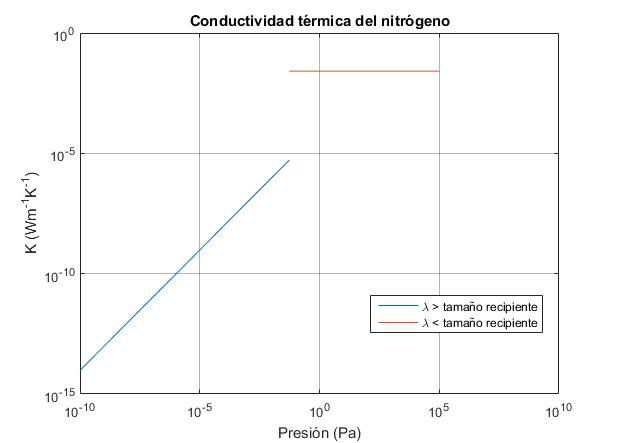
\includegraphics[width=0.55\textwidth]{Imagenes/Unidad/U2/grafp10.jpg}
    \caption{Conductividad térmica del nitrógeno a una temperatura de 300 K. Se considera los casos en que el camino libre medio es menor y mayor que el tamaño del recipiente.}
    \label{fig:my_label}
\end{figure}


\end{enumerate}



\subsection{Otras propiedades}
\begin{enumerate}[resume]
    \item % Pregunta 11
    La absorción es cuando un líquido se disuelve en otro líquido o penetra un sólido. La adsorción es la adhesión de átomos, iones o moléculas de un gas, líquido o sólido disuelto a una superficie. La diferencia entre ellos es que la absorción penetra físicamente mientras que la adsorción se queda en la superficie.  
    \item % Pregunta 12
    Se considera un recipiente cúbico de volumen $V=0.01$ $m^3$. El area del recipiente es $A=6a^2$, donde $a$ es la arista del cubo y su valor es $a=\sqrt[3]{0.01}$. De esta forma $A=0.2785$ $m^2$. Por lo tanto el número de moléculas que forman una monocapa en esta superficie esta dado por
    \begin{equation}
        n_{paredes} = \frac{A}{\sigma} = 3.7 \cdot 10^{18} \quad \text{moléculas}
    \end{equation}
    \item % Pregunta 13
    Por ley de los gases ideales
    \begin{equation}
        n=\frac{PV}{K_{B}T}
    \end{equation}
    Luego, si consideramos $T=300$ K y $V=0.01$ $m^3$ tenemos
    \begin{equation}
        n_{volumen}=\frac{0.01\cdot P}{1.380649 \cdot 10^{-23}\cdot 300} = 2.4 \cdot 10^{18} \cdot P
    \end{equation}
    A presion ambiente se tiene $n_{volumen} = 2.4463 \cdot 10^{23}$ moléculas.
    \item % Pregunta 14
    \begin{equation}
        \frac{n_{paredes}}{n_{volumen}}= \frac{3.713 \cdot 10^{18}}{2.4143 \cdot 10^{18} \cdot P}=\frac{1.5379} {P}
    \end{equation}
    \item % Pregunta 15
    A la presión de 1.5379 pascales el efecto de las partículas en las paredes empieza a predominar sobre el efecto de las partículas en el volumen. 
    \begin{figure}
        \centering
        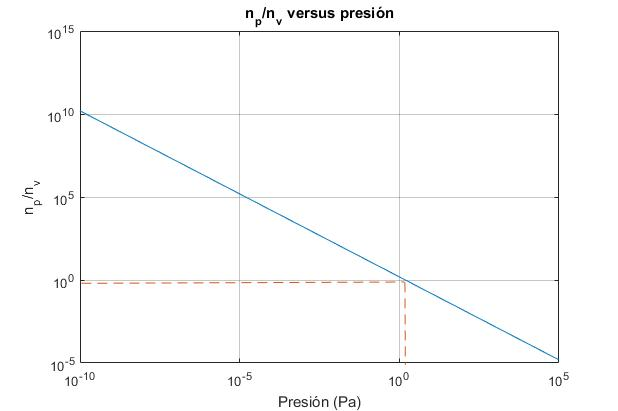
\includegraphics[width=0.55\textwidth]{Imagenes/Unidad/U2/grafp15.jpg}
        \caption{Cociente entre el número de partículas en las paredes y el número de partículas en el volumen en función de la presión.}
        \label{fig:my_label}
    \end{figure}
    
\end{enumerate}


\subsection{Flujo}
\begin{enumerate}[resume]
    \item % Pregunta 16
    \textbf{Flujo turbulento}: también conocido como flujo caótico, corresponde al movimiento de un fluido que se da en forma caótica, en el que las partículas se mueven desordenadamente y las trayectorias de las partículas se encuentran formando remolinos aperiódicos. Ejemplos, flujo detrás de un obstáculo, choque de dos corrientes de agua. Este flujo se produce cuando se comienza a evacuar una cámara de vacío.
    
    \item % Pregunta 17
    \textbf{Flujo viscoso}: en este flujo existen fuerzas de rozamiento entre las moléculas, lo que provoca resistencia a su movimiento. En un tubo las moléculas del fluido se mueven mas rápido cerca del eje longitudinal y mas lento en las paredes. Ejemplo, la miel.
    \\ \\
    \textbf{Flujo laminar}: Se llama flujo laminar o corriente laminar al movimiento de un fluido cuando éste es ordenado, estratificado o suave. En un flujo laminar, el fluido se mueve en láminas paralelas sin entremezclar y cada partícula de fluido sigue una trayectoria suave, llamada línea de corriente. El flujo laminar es típico de fluidos a velocidades bajas o viscosidades altas. Ejemplo, flujo de agua por un tubo a baja velocidad.
    Este flujo se produce cuando se hace vacío grueso y medio.

    \item % Pregunta 18
     % Falta añadir las aplicaciones de los diferentes tipos de flujo a los sistema de vacio. 
    \textbf{flujo molecular}: flujo en el que hay muy poca colisión entre moléculas y por lo tanto el concepto de viscosidad no tiene sentido. Modo de fluir de un gas a través de un conducto en condiciones tales que el recorrido libre medio supera a la dimensión máxima de la sección recta del conducto. El flujo queda totalmente determinado por las colisiones gas-pared. Este flujo se produce cuando se hace alto y ultra alto vacío.
    
    % Falta añadir las aplicaciones de los diferentes tipos de flujo a los sistema de vacio. 

    \item % Pregunta 19
    %Creo q le falta
    \textbf{Flujo de fuga}:
    es un aumento en la presión de un sistema de vacío. Este aumento de presión puede tener dos fuentes:
    \begin{itemize}
        \item una fuga real, dada por defectos del material y/o áreas de conexión, causadas por poros o grietas por estrés mecánico o térmico. También hay moléculas que penetran por permeación desde el exterior.
        
        \item Fuga virtual, no entran moléculas desde el exterior, se produce gas liberado desde las paredes del propio material del recipiente. Es la liberación de un gas que se disolvió, atrapó, congeló o absorbió en el material.
        
    \end{itemize}
\end{enumerate}

\subsection{Aplicaciones}
\begin{enumerate}[resume]
    \item % Pregunta 20  
    \textbf{Física de altas energías}: permite que una partícula alcance altas velocidades ya que disminuye la colisiones con otras moléculas, átomos o partículas.
    \item % Pregunta 21
    \textbf{Bajas temperaturas}:  al haber muy pocas partículas se evita la transmisión de calor por conducción lo que permite desarrollar sistemas aislados térmicamente.
    \\ 
    \textbf{Vaso Dewar}: su estructura principal consta de una doble pared de vidrio, pintada de plateado, y en el espacio intermedio se produce vacío, cuya función principal es evitar la transferencia de energía por convección y conducción, mientras que el plateado permite reflejar la radiación, ya que la plata es un muy buen reflector y tiene baja emisividad. Últimamente se utilizan también fibras de vidrio en el interior para dicho fin.
    \item % Pregunta 22
    \begin{enumerate}
        \item % Parte a
        \textbf{Evaporación de materiales}:  dada la baja presión la temperatura de evaporación del material disminuye. El vacío produce un aumento del camino libre medio de las moléculas del material lo que permite que estas lleguen al substrato. También evita que el aire contamine la superficie del substrato de esta manera se forma una monocapa sin impurezas. 
        \item % Parte b
        Un evaporador térmico que usa un calentador de resistencia eléctrica para derretir el material y elevar su presión de vapor a un rango útil. \textbf{Esto se hace en un alto vacío}, tanto para permitir que el vapor alcance el sustrato sin reaccionar o dispersarse contra otros átomos en fase gaseosa en la cámara, como para reducir la incorporación de impurezas del gas residual en la cámara de vacío. Obviamente, solo los materiales con una presión de vapor mucho más alta que el elemento calefactor pueden depositarse sin contaminar la película.
        \\ 
        Alto vacío: $\mathrm{10^{-3}}-\mathrm{10^{-7}}$ mbar.
        \item % Parte c
        La presión de vapor no depende de la presión ambiente, solo depende de la temperatura y la naturaleza del material que se esta evaporando (aumenta con la temperatura y en general disminuye con el peso molecular).
 
        \item % Parte d
        Al ser baja la presión del recipiente al vapor le tomara mas tiempo alcanzar la presión de saturación por lo que la tasa de condensación crecerá mas lento, es decir habrá mas evaporación. 
        
    \end{enumerate}
    
    \item % Pregunta 23
    \textbf{Ciencia de superficies}: el vacío permite mantener superficies limpias por largos periodos de tiempo lo cual resulta útil en el estudio de la fricción, la adhesión y la corrosión de las superficies.
    \item % Pregunta 24
    Ampolletas, sellado al vacío de alimentos para su conservación. En la fabricación de semiconductores, se requieren ambientes cuidadosamente controlados al vacío.
\end{enumerate}

\subsection{Prevacío}
\begin{enumerate}[resume]
    \item % Pregunta 25
    Consiste en dos paletas cuyos extremos están en permanente contacto con la superficie interna (estator) y están  unidas a un rotor cuyo eje es excéntrico. Esto está diseñado de forma que el volumen de la cámara cambia a medida que el rotor gira. Cuando el aire entra por el puerto de entrada la cámara se agranda, una vez alcanzado el volumen máximo  se inicia la expulsión del aire, al ir disminuyendo el volumen el aire se comprime lo que produce presión en el puerto de salida.
    \begin{figure}
        \centering
        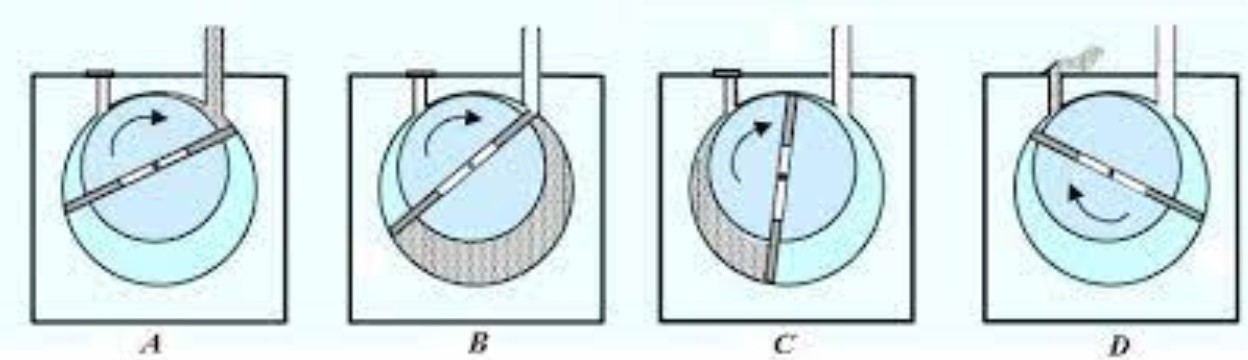
\includegraphics[width=0.8\textwidth]{Imagenes/Unidad/U2/pregunta 25.jpg}
        \caption{Bomba rotatoria de paletas.  }
        \label{pregunta 25}
    \end{figure}
     Animación bomba rotatoria de paletas: \url{https://www.youtube.com/watch?v=gHDVroOnjOI}
    \item % Pregunta 26
    La bomba de dos etapas consiste en dos bombas en serie,es decir la salida de la primera conecta con la entrada de la segunda. La bomba de dos etapas consigue presiones más bajas, y bombea más rápido que la de una etapa.
    \item % Pregunta 27
    El intervalo de presiones en el que funciona la bomba de una etapa es de $\mathrm{10^5}$ a $\mathrm{10^{2}}$ Pa. Mientras que la de dos etapas alcanza una presion del orden de 1 Pa. 
    \item % Pregunta 28
     La bomba scroll consta de dos superficies en forma de espiral, una esta fija y la otra orbita excéntricamente sin girar, atrapando y bombeando o comprimiendo bolsas de fluido entre los rollos. Puede alcanzar una presión del orden de 1 Pa.
     \begin{figure}
         \centering
         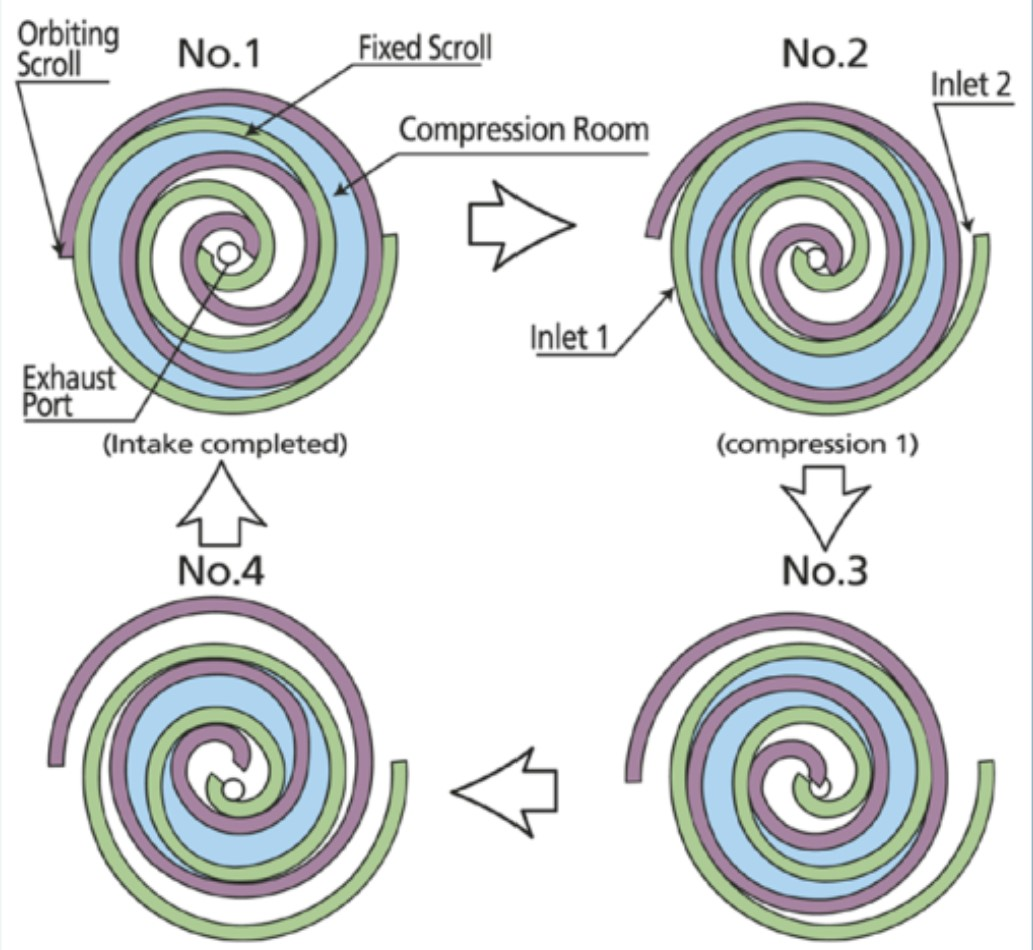
\includegraphics[width=0.4\textwidth]{Imagenes/Unidad/U2/pregunta 28.jpg}
         \caption{Bomba scroll.}
         \label{fig:my_label}
     \end{figure}
     Animación bomba scroll: \url{https://www.youtube.com/watch?v=msd432WvlkI}
\end{enumerate}


\subsection{Alto Vacío y Bombas difusoras}
\begin{enumerate}
\setcounter{enumi}{29}
    \item % Pregunta 30
    En la bomba de difusión se calienta aceite, el vapor del aceite sube por la chimenea y es expulsado en dirección descendente. De esta forma las moléculas de gas de la cámara son llevadas hacia abajo por la transferencia de momentum cuando colisionan con las moléculas de aceite. El aceite choca con las paredes que están refrigeradas y se condensa volviendo a la caldera, mientras las moléculas son succionadas por una bomba de respaldo. Estas bombas pueden alcanzar presiones de $\mathrm{10^{-9}} \sim \mathrm{10^{-10}}$ Pa.
    
    \item % Pregunta 31
    La bomba difusora no tiene capacidad de descargar directamente a la atmósfera, por eso debe ser respaldada por una bomba mecánica que mantenga una presión de salida suficiente para evacuar las moléculas de gas. Esta se necesita para que no hayan colisiones de las moléculas de aceita y se produzca un reflujo de aceite hacia la cámara, se requiere un prevacío que alcance una presión en torno a 25-75 Pa. Si la presión no es suficientemente baja el chorro de aceite no logra alcanzar la pared del recipiente y se produce reflujo. \\ \\
    Animación: \url{https://www.youtube.com/watch?v=ubno1kNtxIQ}
    
    \item % Pregunta 32
    \begin{enumerate}
        \item % Parte a
        \textbf{Corriente de retorno}: corresponde al flujo de aceite hacia la cámara de vacío debido a colisiones que hacen ascender a las moléculas de aceite, esta se puede producir por 
        \begin{itemize}
            \item evaporación del fluido condensado en las paredes superiores de la bomba.
            \item ebullición prematura del aceite condensado antes de entrar en la caldera.
            \item la sobreexcitación del vapor de aceite en el chorro superior  fugas en la tapa del chorro.
            \item colisión de las moléculas de aceite con las moléculas del gas.
        \end{itemize}
        
        \item % Parte b
        \textbf{Pantalla}: son paneles ubicados entre la cámara y la boca de la bomba que disminuyen la corriente de retorno obstruyendo el flujo de las moléculas de aceite hacia la cámara.

        \item % Parte c
        \textbf{Trampa criogénica}: es un dispositivo que condensa el vapor de aceite. Con él se puede evitar la corriente de retorno, además el aceite condensado baja por las paredes arrastrando consigo las moléculas de gas. Su objetivo es evitar que los vapores contaminen el experimento.
    \end{enumerate}
\end{enumerate}

\subsection{Tipos de Vacío}
\begin{enumerate}
\setcounter{enumi}{33}
    \item % Pregunta 34
    \begin{figure}
        \centering
        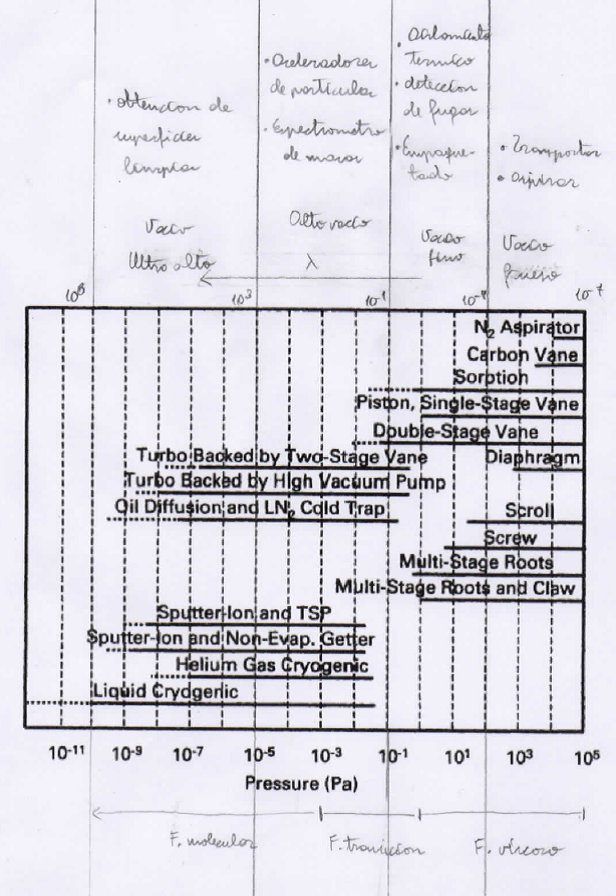
\includegraphics[width=0.7\textwidth]{Imagenes/Unidad/U2/p34.png}
        \caption{Tabla-gráfico con tipos de vacío, flujos, bombas y aplicaciones típicas en un rango de presión correspondiente.}
        \label{fig:my_label}
    \end{figure}
  
\end{enumerate}


\subsection{Medición de Presiones}

\begin{enumerate}
    \setcounter{enumi}{34}
    \item % Pregunta 35
    \textbf{Medición directa}: se mide directamente la fuerza de una partícula incidente sobre una superficie. \\ \\
    \textbf{Medición indirecta}: se miden propiedades del gas que dependen de la presión. 
    \item % Pregunta 36
    Un manómetro sencillo, consiste en un tubo doblado en forma de U que contiene un líquido, generalmente mercurio, un extremo está abierto a la atmósfera y el otro está conectado al depósito donde está el fluido al cual se quiere medir su presión. El líquido del tubo se desplaza hasta alcanzar un equilibrio, en el equilibrio se puede determinar la presión en función de la diferencia de las alturas de las columnas.
    \item % Pregunta 37
    Consiste en un alambre que es calentado por una corriente constante y expuesto al medio donde se quiere medir la presión, a medida que la presión incrementa la temperatura del alambre disminuye (al transferir energía cinética a las partículas el alambre se enfría) , esta disminución de temperatura se mide a través de una termocupla.
    \\
    Una \textbf{termocupla} es un sensor para medir la temperatura. Consiste en dos metales diferentes unidos por un extremo. Cuando la unión de los dos metales se calienta o enfría se produce un voltaje que se puede correlacionar con la temperatura.
    \item % Pregunta 38
    Un manómetro de cátodo frío ioniza el gas en el sistema aplicando un voltaje muy alto entre un ánodo en forma de anillo y un cátodo formado por dos placas paralelas a ambos lados del anillo. por la aplicación de un campo magnético se logra que los electrones sigan trayectorias helicoidales, lo que aumenta el choque con las moléculas de gas. la corriente de iones que se forma depende del potencial de ionización y del número de choque con los electrones que a su vez depende de la presión del sistema, por lo que se usa la corriente de ionización como medida de la presión.
    Animación: \url{https://youtu.be/TG9vtKK-LLw}
\end{enumerate}


\subsection{Evaporación de un material}

\begin{enumerate}
    \setcounter{enumi}{39}
    %\item % Pregunta 39
    %\item % Pregunta 40
    \begin{figure}
        \centering
        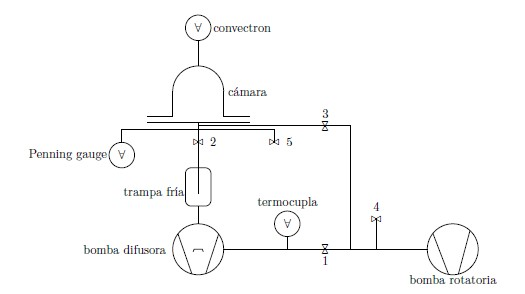
\includegraphics[width=0.7\textwidth]{Imagenes/Unidad/U2/p40.jpg}
        \caption{Diagrama montaje experimental. Pregunta 39}
        \label{fig:my_label}
    \end{figure}
    \item % Pregunta 40
    \begin{enumerate}
        \item $600$ ºC
        \item $1010$ ºC
    \end{enumerate}
\end{enumerate}